\section{Kernel Interpolation}

\subsection{Inspiration from $\delta$ Function}

\subsubsection{Dirac $\delta$ Function}

$\delta$ function is a function that is zero everywhere except at the origin, 
and its integral is 1. It is defined as
\begin{equation}
    \begin{aligned}
        \delta(x) = 
        \begin{cases}
            +\infty, & x = 0 \\
            0, & x \neq 0
        \end{cases}
        \quad \text{and} \quad
        \int_{-\infty}^{+\infty} \delta(x) \mathrm{d}x = 1
    \end{aligned}
\end{equation}

This function has a wide application in physics, 
especially in quantum mechanics. 
Such function has only math definition instead of detailed physical meaning.

$\delta$ function has 2 main properties:
\begin{itemize}
    \item $\delta(x) = 0, \forall x \neq 0$, which is called \textbf{locality} or \textbf{compact support}.
    \item $\int_{-\infty}^{+\infty} f(\xi) \delta(x - \xi)\mathrm{d}\xi = f(x)$, which is called \textbf{sifting property}.
\end{itemize}

These 2 properties are the key to the application of SPH method.

\begin{figure}[H]
    \centering
    \begin{tikzpicture}
        \draw[->] (-3, 0) -- (3, 0) node[right] {$x$};
        \draw[->] (0, -0.5) -- (0, 2) node[above] {$\delta(x)$};
        \draw[domain=-3:-0.1, samples=100] plot(\x, {0});
        \draw[domain=0.1:3, samples=100] plot(\x, {0});
        \draw[domain=-0.1:0.1, samples=100] plot(\x, {1.5});
        \draw (-0.1, 1.5) node[left] {$+\infty$};
    \end{tikzpicture}
    \caption{Dirac $\delta$ function}
    \label{fig:delta_function}
\end{figure}

In high-dimensional space, $\delta$ function is defined as
\begin{equation}
    \delta(\vec{r})=
    \begin{cases}
        +\infty, & \vec{r} = 0 \\
        0, & \vec{r} \neq 0
    \end{cases}
    \quad \text{and} \quad
    \int_{-\infty}^{+\infty} \delta(\vec{r}) \mathrm{d}\vec{r} = 1
\end{equation}
also, the sifting property is
\begin{equation}
    \int_{-\infty}^{+\infty} f(\vec{r}^\prime) \delta(\vec{r} - \vec{r}^\prime)\mathrm{d}\vec{r}^\prime = f(\vec{r})
\end{equation}

An inspiration comes out from the properties, 
which proposes the idea of using a $\delta$-like function to interpolate the physical quantities.

\subsubsection{$\delta$-like Function}

$\delta$-like function is a function that is zero everywhere except a small region around the origin,
and its integral is 1. It is defined as:
\begin{equation}
    \begin{aligned}
        W(x,h) = 
        \begin{cases}
            f(x), & |x| \leq h \\
            0, & |x| > h
        \end{cases}
        \quad \text{and} \quad
        \int_{-\infty}^{+\infty} W(x,h) \mathrm{d}x = 1
    \end{aligned}
\end{equation}
in high dimensional space, $W(\vec{r},h)$ is defined as
\begin{equation}
    \begin{aligned}
        W(\vec{r},h) = 
        \begin{cases}
            f(\vec{r}), & |\vec{r}| \leq h \\
            0, & |\vec{r}| > h
        \end{cases}
        \quad \text{and} \quad
        \int_{-\infty}^{+\infty} W(\vec{r},h) \mathrm{d}\vec{r} = 1
    \end{aligned}
\end{equation}

Here, $h$ is called \textbf{smoothing kernel length}. 
Also it's written as $h$, 
a radius ratio $t$ is often introduced to represent the kernel length $t h$ in application.
$t$ is called \textbf{smoothing kernel ratio}.
In equation formula, we use $h$ to represent the smoothing kernel length for simplicity.

A simple $\delta$-like function is the Gaussian function (1D):
\begin{equation}
    W(x,h) = \frac{1}{\sqrt{2\pi}h} \exp\left(-\frac{x^2}{2h^2}\right)
\end{equation}

\begin{figure}[H]
    \centering
    \begin{tikzpicture}
        \draw[->] (-3, 0) -- (3, 0) node[right] {$x$};
        \draw[->] (0, -0.5) -- (0, 3) node[above] {$W(x,h)$};
        \draw[domain=-3:-0.1, samples=100] plot(\x, {0});
        \draw[domain=0.1:3, samples=100] plot(\x, {0});
        \draw[domain=-0.1:0.1, samples=100] plot(\x, {1.5});
        \draw[domain=-3:3, samples=100] plot(\x, {exp(-(\x*\x)/0.2)/sqrt(2*pi)/0.2});
    \end{tikzpicture}
    \caption{$\delta$-like function: Gaussian function}
    \label{fig:delta_like_function_gaussian}
\end{figure}

$\delta$ function can be seen as a limit of Gaussian function when $h \rightarrow 0$:
\begin{equation}
    \lim_{h \rightarrow 0} W(x,h) = \delta(x)
\end{equation}

Although $\delta$-like function is not a real $\delta$ function, 
in numerical respect, 
it shares the same properties with $\delta$ function and can be used to interpolate the physical quantities.

\subsubsection{Let $\delta$-like Function Share Properties with $\delta$ Function}

$\delta$-like function shares the same properties with $\delta$ function:
\begin{itemize}
    \item $W(x,h) = 0, \forall |x| > h$, which is called \textbf{locality} or \textbf{compact support}.
    \item $\int_{-\infty}^{+\infty} f(\xi) W(x - \xi,h)\mathrm{d}\xi = f(x)$, which is called \textbf{sifting property}.
    \item $\int_{-\infty}^{+\infty} W(x,h) \mathrm{d}x = 1$, which is called \textbf{normalization}.
\end{itemize}

In $d$-dimensional space, 
$W(\vec{r},h)$ is zero everywhere except a $d$-dimensional sphere with radius $h$ around the origin.
With sifting property, 
$f(\vec{r})$'s value can be interpolated by $f(\vec{r}^\prime)$ distributed in a sphere with radius $h$ around $\vec{r}$.

\subsection{Kernel Function}

\subsubsection{Definition of Kernel Function}

Kernel function is a function that is zero everywhere except a small region around the origin,
and its integral is 1. It is defined as:
\begin{equation}
    \begin{aligned}
        W(\vec{r},h) = 
        \begin{cases}
            f(\vec{r}), & |\vec{r}| \leq h \\
            0, & |\vec{r}| > h
        \end{cases}
        \quad \text{and} \quad
        \int_{-\infty}^{+\infty} W(\vec{r},h) \mathrm{d}\vec{r} = 1
    \end{aligned}
\end{equation}

Here, $h$ is called \textbf{smoothing kernel length}.
It is an even function, as long as $|\vec{r}_1| = |\vec{r}_2|$, 
we have:
\begin{equation}
    W(\vec{r}_1, h) = W(\vec{r}_2, h)
\end{equation}

Usually, $W(\vec{r},h)$ is given by form of:
\begin{equation}
    W(\vec{r},h) = W(q) = W\left(\frac{r}{h}\right)\quad 
    r = |\vec{r}| = \sqrt{\vec{r}\cdot\vec{r}}=\sqrt{\sum_j x_j^2}
\end{equation}

\subsubsection{Derivation of Kernel Function}

Let's consider kernel function's derivation in $x_j$ direction:
\begin{equation}
    \begin{aligned}
        \frac{\partial W}{\partial x_j}&=
        \frac{\partial W}{\partial q}\frac{\partial q}{\partial r}\frac{\partial r}{\partial x_j}\\
        &=W^\prime \frac{1}{h}\frac{x_j}{r}
    \end{aligned}
\end{equation}

Thus $\nabla W$ is:
\begin{equation}
    \nabla W = \frac{1}{h} W^\prime \frac{\vec{r}}{r}
    = \frac{1}{h} W^\prime \hat{\vec{r}}
\end{equation}
$\hat{\vec{r}}$ is the unit vector of $\vec{r}$.

$\nabla W$ has the same direction with $\vec{r}$, and:
\begin{equation}
    \vec{r}\cdot \nabla W = \frac{r}{h} W^\prime\quad
    |\nabla W| = \left|\frac{1}{h} W^\prime\right|
\end{equation}
it's worth noting that $\nabla{W}$ will meet a singularity when $\vec{r}=\vec{0}$.

\subsection{Kernel Interpolation}

\subsubsection{Physical Quantity Kernel Interpolation}

As is discussed above, 
$\delta$-like function can be used to interpolate the physical quantities.
The interpolation formula is:
\begin{equation}
    f(\vec{r}) = \int_{-\infty}^{+\infty} f(\vec{r}^\prime) W(\vec{r} - \vec{r}^\prime,h)\mathrm{d}\vec{r}^\prime
\end{equation}

Now, let's consider the space domain discretized into particles, 
each particle is a material point with mass $m_i$ and position $\vec{r}_i$.

\begin{figure}[H]
    \centering
    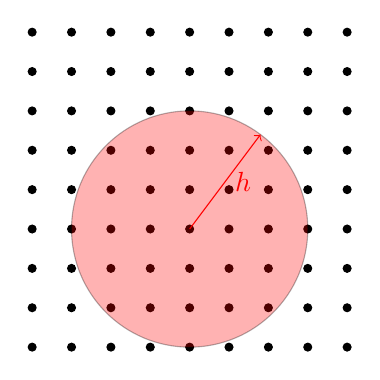
\begin{tikzpicture}
        \foreach \x in {0, 1, 2, 3, 4, 5, 6, 7, 8}
            \foreach \y in {0, 1, 2, 3, 4, 5, 6, 7, 8}
                \filldraw (0.5*\x, 0.5*\y) circle (0.05);
        \filldraw[fill=red, opacity=0.3] (0.5*4, 0.5*3) circle (1.5);
        \draw[->, red] (0.5*4, 0.5*3) -- (0.5*4+0.9, 0.5*3+1.2);
        \node[red] at (0.5*4+0.68, 0.5*3+0.6) {$h$};
    \end{tikzpicture}
\end{figure}

These particles have a scalar physical quantity $A_i$ and a vector physical quantity $\vec{v}_i$.
In SPH method, there values on particle $i$ can be interpolated with help of kernel function by 
particles $j$ near particle $i$:
\begin{equation}
    \begin{aligned}
        A_i &= \sum_j A_j W(\vec{r}_i - \vec{r}_j, h) \Delta V_j \\
        \vec{v}_i &= \sum_j \vec{v}_j W(\vec{r}_i - \vec{r}_j, h) \Delta V_j
    \end{aligned}
\end{equation}
$\Delta V_j$ is the volume of particle $j$, and $|\vec{r}_i - \vec{r}_j| \leq h$. 
As particle $j$'s mass $m_j$ and density $\rho_j$ are known, volume $\Delta V_j$ is substituted as below:
\begin{equation}
    \begin{aligned}
        A_i &= \sum_j \frac{m_j}{\rho_j} A_j W(\vec{r}_i - \vec{r}_j, h) \\
        \vec{v}_i &= \sum_j \frac{m_j}{\rho_j} \vec{v}_j W(\vec{r}_i - \vec{r}_j, h)
    \end{aligned}
\end{equation}

For simplicity, 
denote $W(\vec{r}_i - \vec{r}_j, h)$ as $W_{ij}$ as the kernel function is specified by $h$.
\begin{equation}
    \begin{aligned}
        A_i &= \sum_j \frac{m_j}{\rho_j} A_j W_{ij} \\
        \vec{v}_i &= \sum_j \frac{m_j}{\rho_j} \vec{v}_j W_{ij}
    \end{aligned}
\end{equation}

\subsubsection{Derivation of Kernel Interpolation}

The derivation of kernel interpolation is based on the sifting property of $\delta$-like function.
Let's consider a scalar's gradient value first:

\begin{equation}
    \begin{aligned}
        \nabla A(\vec{r}) &= 
        \int_{\Omega} \nabla A(\vec{r}^\prime) W(\vec{r} - \vec{r}^\prime,h)\mathrm{d}\vec{r}^\prime \\
        &\mathop{=}^{\text{symmetry}}
        \int_{\Omega} \nabla A(\vec{r}^\prime) W(\vec{r}^\prime-\vec{r},h)\mathrm{d}\vec{r}^\prime\\
        &\mathop{=}^{\text{Green's theorem}}
        \int_{\partial\Omega} A(\vec{r}^\prime) \vec{n} W(\vec{r}^\prime-\vec{r},h)\mathrm{d}\vec{r}^\prime
        - \int_{\Omega} A(\vec{r}^\prime) \nabla W(\vec{r}^\prime-\vec{r},h)\mathrm{d}\vec{r}^\prime\\
        &\mathop{=}^{\text{compact support}}
        - \int_{\Omega} A(\vec{r}^\prime) \nabla W(\vec{r}^\prime-\vec{r},h)\mathrm{d}\vec{r}^\prime\\
        &\mathop{=}^{\text{anti-symmetry}}
        \int_{\Omega} A(\vec{r}) \nabla W(\vec{r}-\vec{r}^\prime,h)\mathrm{d}\vec{r}^\prime\\
    \end{aligned}
\end{equation}

In the derivation, 
$\Omega$ is the space domain of the scalar $A(\vec{r})$, 
$\partial\Omega$ is the boundary of $\Omega$. 
For compact support, 
boundary part integral is zero.
In discretized form, 
such integral can be written as:
\begin{equation}
    \nabla A_i = \sum_j \frac{m_j}{\rho_j} A_j \nabla W(\vec{r}_i - \vec{r}_j, h)
\end{equation}

$\nabla W(\vec{r}_i - \vec{r}_j, h) = -\nabla W(\vec{r}_j - \vec{r}_i, h)$ for symmetry. 
In other people's papers and book, they usually denote $\nabla W(\vec{r}_i - \vec{r}_j, h)$ as $\nabla_i W_{ij}$. 
Here, we use $\nabla W_{ij}$ for simplicity:
\begin{equation}
    \nabla A_i = \sum_j \frac{m_j}{\rho_j} A_j \nabla W_{ij}
\end{equation}

However, this form of gradient is not that accurate. 
Now we consider a more accurate form of gradient. 
Multiply a scalar $\phi$ to the gradient:
\begin{equation}
    \phi\nabla A = \nabla(\phi A) - A\nabla\phi
\end{equation}

Let $\phi = \frac{1}{\rho}$, 
then:
\begin{equation}
    \begin{aligned}
        \frac{1}{\rho}\nabla A &= \nabla\left(\frac{A}{\rho}\right) - A\nabla\left(\frac{1}{\rho}\right)\\
        &=
        \nabla\left(\frac{A}{\rho}\right) + A\frac{\nabla\rho}{\rho^2}
    \end{aligned}
\end{equation}

In particle discretized form, we will have an approximation of $\frac{\nabla p}{\rho}$:
\begin{equation}
    \left(\frac{1}{\rho}\nabla A\right)_i
    =
    \sum_j m_j
    \left(
        \frac{A_j}{\rho_j^2}
        +
        \frac{A_i}{\rho_i^2}
    \right)\nabla W_{ij}
\end{equation}

What is worth noting
is that the choice of $\phi$ is not unique, 
different choice of $\phi$ will lead to different form of particle-discretized gradient.

For vector physical quantity $\vec{v}$,
we focus on the divergence of $\vec{v}$ and laplacian of $\vec{v}$.

\begin{equation}
    \begin{aligned}
        \nabla\cdot \vec{v} &=
        \int_{\Omega} \nabla\cdot \vec{v}(\vec{r}^\prime) W(\vec{r} - \vec{r}^\prime,h)\mathrm{d}\vec{r}^\prime \\
        &\mathop{=}^{\text{symmetry}}
        \int_{\Omega} \nabla\cdot \vec{v}(\vec{r}^\prime) W(\vec{r}^\prime-\vec{r},h)\mathrm{d}\vec{r}^\prime\\
        &\mathop{=}^{\text{Green's theorem}}
        \int_{\partial\Omega} \vec{v}(\vec{r}^\prime) \cdot \vec{n} W(\vec{r}^\prime-\vec{r},h)\mathrm{d}\vec{r}^\prime
        - \int_{\Omega} \vec{v}(\vec{r}^\prime) \cdot \nabla W(\vec{r}^\prime-\vec{r},h)\mathrm{d}\vec{r}^\prime\\
        &\mathop{=}^{\text{compact support}}
        - \int_{\Omega} \vec{v}(\vec{r}^\prime) \cdot \nabla W(\vec{r}^\prime-\vec{r},h)\mathrm{d}\vec{r}^\prime\\
        &\mathop{=}^{\text{anti-symmetry}}
        \int_{\Omega} \vec{v}(\vec{r}) \cdot \nabla W(\vec{r}-\vec{r}^\prime,h)\mathrm{d}\vec{r}^\prime\\
    \end{aligned}
\end{equation}

In discretized form:
\begin{equation}
    \nabla\cdot \vec{v}_i = \sum_j \frac{m_j}{\rho_j} \vec{v}_j \cdot \nabla W_{ij}
\end{equation}

It's the same problem that inaccuracy still exists in divergence of $\vec{v}$, 
thus we consider a more accurate form.
Multiply a scalar $\phi$ to the divergence:
\begin{equation}
    \phi\nabla\cdot \vec{v} = \nabla\cdot(\phi \vec{v}) - \vec{v}\cdot\nabla\phi
\end{equation}

Let $\phi = \rho$, 
then:
\begin{equation}
    \begin{aligned}
        \rho\nabla\cdot \vec{v} &= \nabla\cdot(\rho \vec{v}) - \vec{v}\cdot\nabla\rho\\
        &=
        \nabla\cdot(\rho \vec{v}) - \vec{v}\cdot\nabla\rho
    \end{aligned}
\end{equation}

In particle discretized form, we will have an approximation of $\rho\nabla\cdot \vec{v}$:
\begin{equation}
    \left(\rho\nabla\cdot \vec{v}\right)_i
    =
    \sum_j m_j
    (\vec{v}_j - \vec{v}_i)\cdot\nabla W_{ij}
    =-\sum_j m_j \vec{v}_{ij}\cdot\nabla W_{ij}
\end{equation}

$\vec{v}_{ij} = \vec{v}_i - \vec{v}_j$ is the velocity difference between particle $i$ and $j$.
For laplacian of $\vec{v}$,
the formula is much more complicated, 
of which the form will be given by detailed description in SPH method section.

\subsection{Frequently-used Kernel Functions}

\subsubsection{Cubic Spline Kernel Function}

Cubic spline kernel function is a piecewise function,
which is defined as:
\begin{equation}
    W(q)=\sigma_3
    \begin{cases}
        \begin{aligned}
            1-\frac{3}{2}q^2\left(1-\frac{q}{2}\right)\quad &0\leq q \leq 1 \\
            \frac{1}{4}(2-q)^3\quad &1\leq q \leq 2 \\
            0\quad &q > 2
        \end{aligned}
    \end{cases}\quad
    \sigma_3=
    \begin{cases}
        \begin{aligned}
            \frac{2}{3h} \quad &d=1 \\
            \frac{10}{7\pi h^2} \quad &d=2 \\
            \frac{1}{\pi h^3} \quad &d=3
        \end{aligned}
    \end{cases}
\end{equation}

\subsubsection{Gaussian Kernel Function}

Gaussian kernel function is a $\delta$-like function,
which is defined as:
\begin{equation}
    W(q)=
    \begin{cases}
        \begin{aligned}
            \sigma_g e^{-q^2}\quad &q \geq 0 \\
            0\quad &q < 0
        \end{aligned}
    \end{cases}\quad
    \sigma_g=
    \begin{cases}
        \begin{aligned}
            \frac{1}{\pi^{1/2}h} \quad &d=1 \\
            \frac{1}{\pi h^2} \quad &d=2 \\
            \frac{1}{\pi^{3/2} h^3} \quad &d=3
        \end{aligned}
    \end{cases}
\end{equation}

\subsubsection{Wendland Kernel Function}

Wendland kernel function is a $\delta$-like function, 
for WendlandC2 kernel function:
\begin{equation}
    W(q)=\alpha_d
    \begin{cases}
        \begin{aligned}
            \left(1-\frac{q}{2}\right)^4(2q+1)\quad &0\leq q \leq 2 \\
            0\quad &q > 2
        \end{aligned}
    \end{cases}\quad
    \alpha_d=
    \begin{cases}
        \begin{aligned}
            \frac{7}{4\pi h^2} \quad &d=2 \\
            \frac{21}{16\pi h^3} \quad &d=3
        \end{aligned}
    \end{cases}
\end{equation}

Another Wendland kernel function is WendlandC4 kernel function:
\begin{equation}
    W(q)=\alpha_d
    \begin{cases}
        \begin{aligned}
            \left(1-\frac{q}{2}\right)^6
            \left(\frac{35}{12}q^2+3q+1\right)\quad &0\leq q \leq 2 \\
            0\quad &q > 2
        \end{aligned}
    \end{cases}\quad
    \alpha_d=
    \begin{cases}
        \begin{aligned}
            \frac{9}{4\pi h^2} \quad &d=2 \\
            \frac{495}{256\pi h^3} \quad &d=3
        \end{aligned}
    \end{cases}
\end{equation}

\subsection{Reflection on Kernel Interpolation: Reduced to Traditional FDM}

As a new researcher to SPH method, 
the biggest question in my mind is that 
why the kernel interpolation can accurately interpolate the physical quantities. 
Kernel interpolation is more like a mathematical trick, rather than a numerical tool.

However, after coding and testing a simple SPH demo, 
I began to understand that kernel interpolation actually provide a cheap way to calculate a 
particle's contribution to scalar physical quantity and gradient around its neighbourhood.

Let's consider a particle $i$ in 1-D space, and a kernel function as below.

\begin{figure}[H]
    \centering
    \begin{tikzpicture}
        \draw[-] (-1,0)--(0,5)--(1,0);
        \draw[->] (-4,0)--(4,0) node[right] {$x$};
        \draw[->] (0,-0.5)--(0,6) node[above] {$W(x,h)$};
        \node at (1,-0.2) {$+h$};
        \node at (-1,-0.2) {$-h$};

        \node at (0.2, 5) {$u_i$};
        \node at (1.2, 5) {$u_{i+1}$};
        \node at (-0.8, 5) {$u_{i-1}$};

        \draw[dashed] (0,0)--(1,5)--(2,0);
        \draw[dashed] (0,0)--(-1,5)--(-2,0);
    \end{tikzpicture}
\end{figure}

\begin{equation}
    W(x,h)=
    \begin{cases}
        \begin{aligned}
            &-\frac{|x|}{h^2}+\frac{1}{h}\quad |x| \leq h \\
            &0 \quad |x| > h
        \end{aligned}
    \end{cases}
    \quad h \ll 1
\end{equation}

$W(x,h)$'s integral is 1:
\begin{equation}
    \int_{-h}^{+h} \left(-\frac{|x|}{h^2}+\frac{1}{h}\right)\mathrm{d}x = 1
\end{equation}

Particles of $i-1$, $i$ and $i+1$, has linear density $\rho_0$ and mass 
$m_j = \rho_0 h, j=i-1,i,i+1$.
\begin{equation}
    W(0,h)\frac{m_i}{\rho_0} = 1
\end{equation}

When $i$ particle and $j(=i+1)$ particle has a distance $h$, 
the interpolation will reduced to:
\begin{equation}
    \begin{aligned}
        u(x) = \left(1-\frac{x}{h}\right)u_i + \frac{x}{h}u_{i+1}\quad 
        0\leq x \leq h
    \end{aligned}
\end{equation}

And the gradient of $u(x)$ is:
\begin{equation}
    \begin{aligned}
        \frac{\partial u}{\partial x} = \frac{u_{i+1}-u_i}{h}
        =
        \partial_x W_i\frac{m_i}{\rho_0} u_i + \partial_x W_{i+1}\frac{m_{i+1}}{\rho_0} u_{i+1}
    \end{aligned}
\end{equation}

It seems that SPH method is reduced to a simple linear interpolation like finite difference method.

As 2 particles' relative distance changes, 
such kind of linear kernel function will cause trouble. 
It only works when the distacne is $h$. 
Thus
a more complicated kernel function is needed to fit for different distance.
That's the reason why kernel function can approximate the physical quantities and gradient.